% !TeX spellcheck = en_GB
% ***************************************************** %
\section{Results}\label{subsc:res}
% ***************************************************** %

In order to run the algorithms, we first explore the \emph{solution space} using the \texttt{multi-start} meta-heuristic on different TSP instances. he considered problems have different sizes: $N=\numlist{10;15;20;30}$ on circular and random layouts.

Exploring the solution space means to empirically find the \emph{energy landscape}, that is the distribution of $f(x^\ast)$ for each local minima that the algorithms have found. Figure~\vref{fig:res-energy} shows these results.

We then select one of the problem instances and solve




the problem and we show the results in figures~\ref{fig:res-local-search} and~\vref{fig:res-sim-annealing}.

Results show that local search easily gets trapped in local minima, especially the \texttt{swap} method, while \texttt{reverse} proves to be a better choice, however both need more iterations

Simulated annealing requires a great length of the Markov chain


% ***************************************************** %
\subsection{Energy landscape}\label{subsc:energy-land}
% ***************************************************** %

The energy landscape means to empirically find the distribution of the objective function for different TSP instances. Using a multi-start method on a local search and simulated annealing we keep track of each $x^\ast$ that the algorithms reach and then the histogram using each $f(x^\ast)$ is plotted.

See figure

% il panorama dell'energia è dipendente dal numero di iterazioni che si lasciano fare all'algoritmo


\begin{figure}
\centering
\subfloat[\emph{Local search, circular layout}]%
	{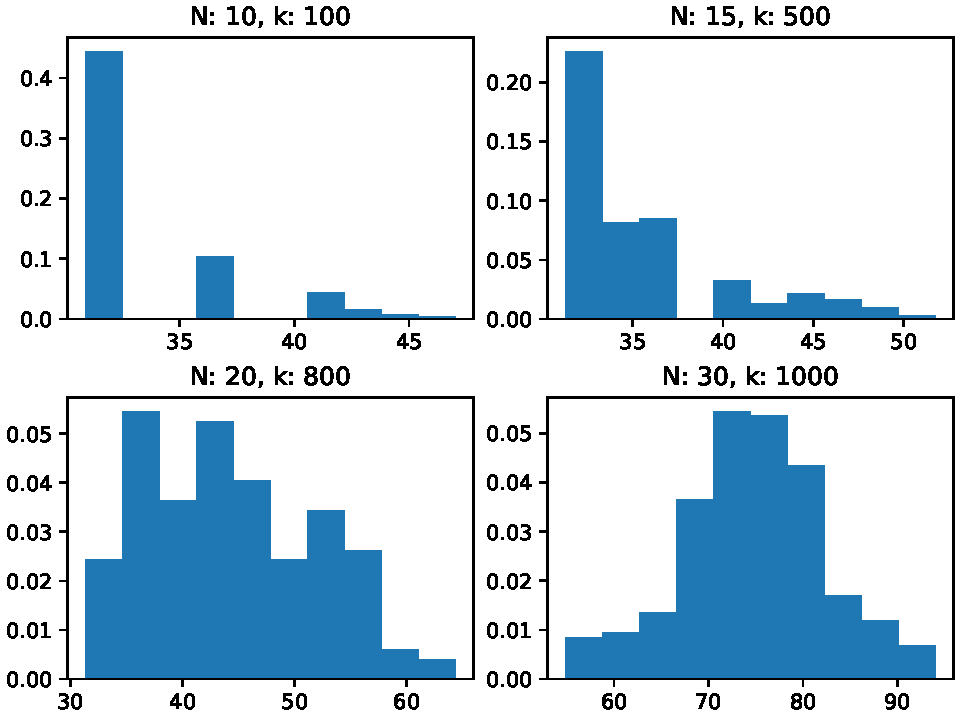
\includegraphics[width=0.49\textwidth]{circle-reverse-energy}} \,
\subfloat[\emph{Local search, random layout}]%
	{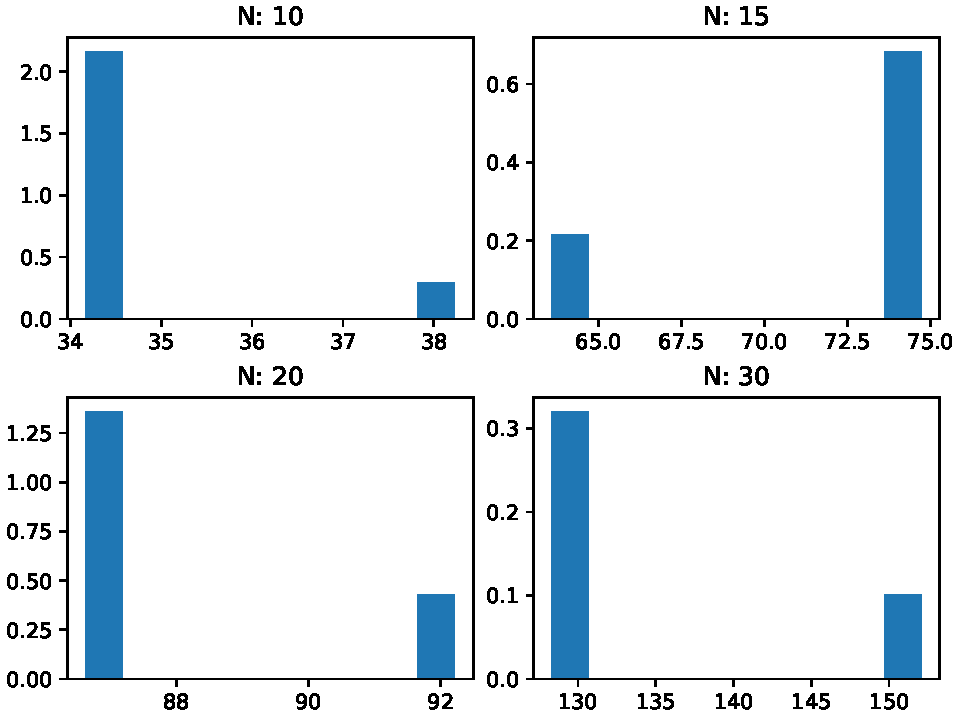
\includegraphics[width=0.49\textwidth]{rand-reverse-energy}} % \\
%\subfloat[\emph{Local search with \texttt{reverse} method}]%
%	{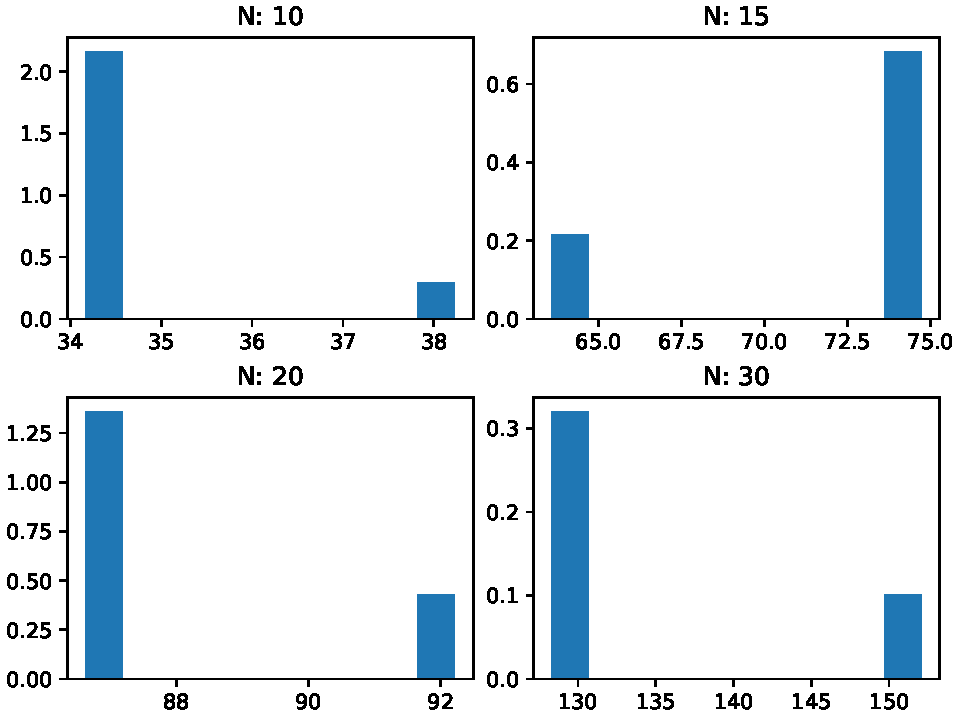
\includegraphics[width=0.49\textwidth]{rand-reverse-energy}} \,
%\subfloat[\emph{Simulated annealing}]%
%	{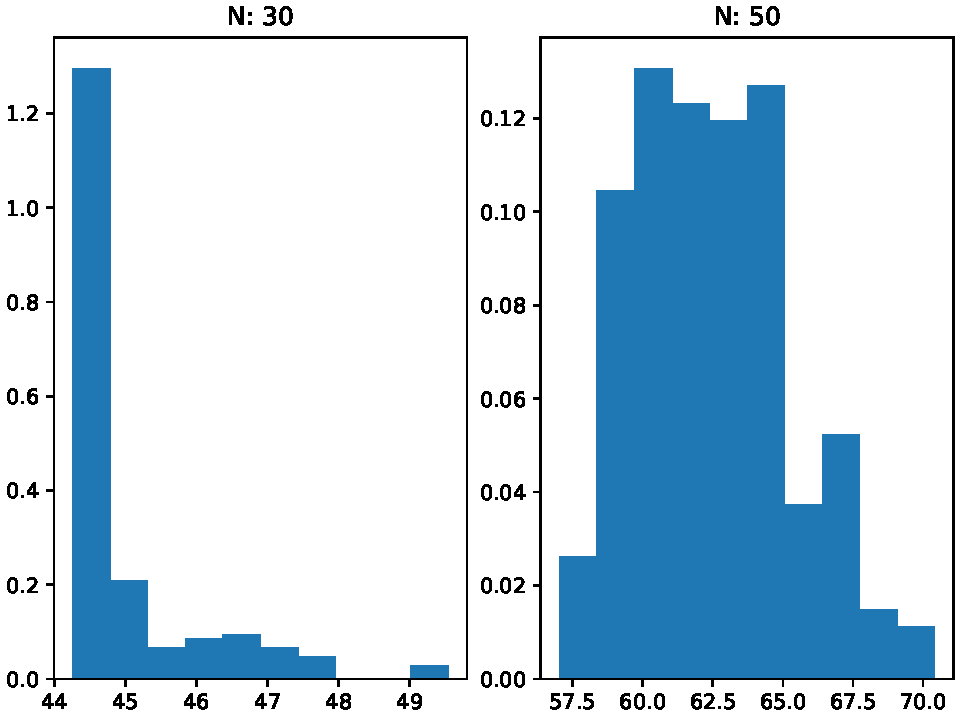
\includegraphics[width=0.49\textwidth]{rand-annealing-energy}}
\caption{Local search with \texttt{reverse} method and SA energy landscapes for different TSP instances}
\label{fig:res-energy}
\end{figure}



\begin{figure}
\centering
\subfloat[\emph{\texttt{swap} method on circular layout}]%
	{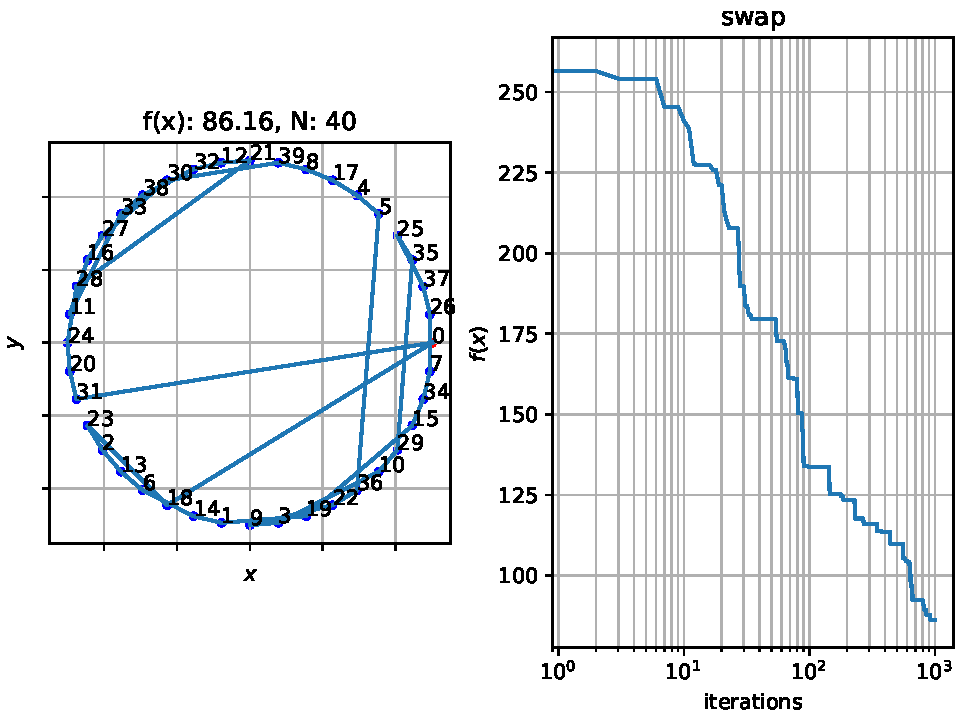
\includegraphics[width=0.49\textwidth]{circle-swap}} \,
\subfloat[\emph{\texttt{reverse} method on circular layout}]%
	{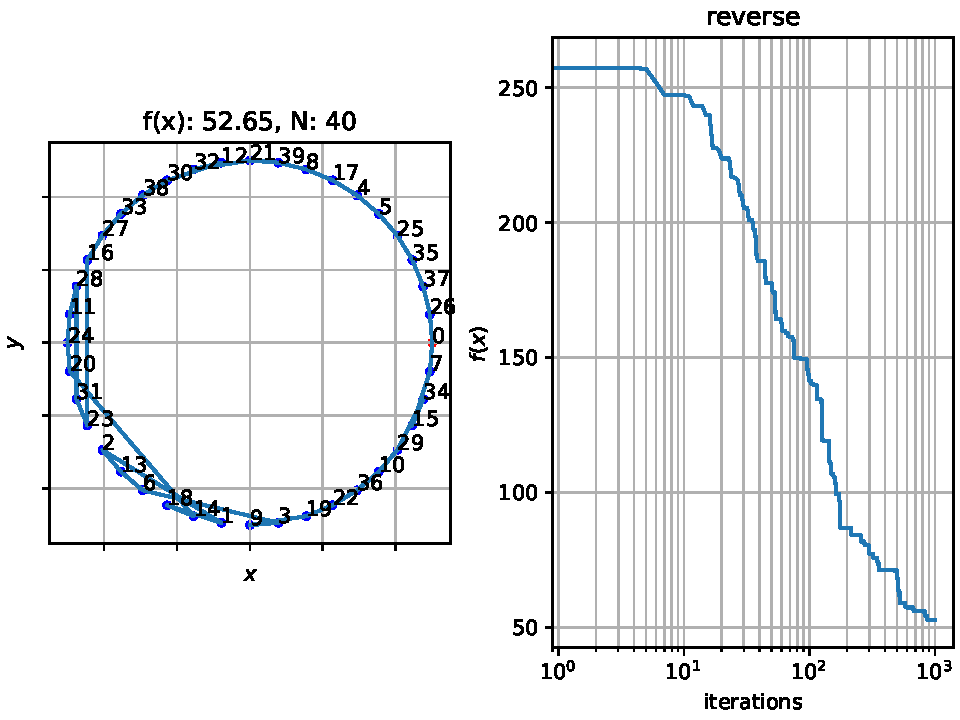
\includegraphics[width=0.49\textwidth]{circle-reverse}} \\
\subfloat[\emph{\texttt{swap} method on random layout}]%
	{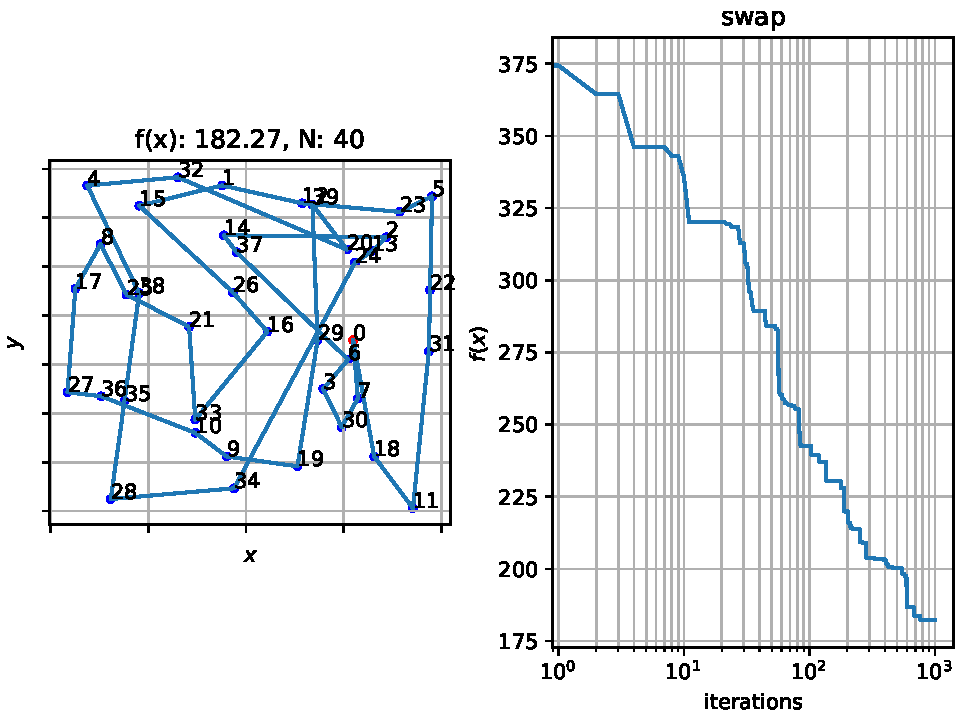
\includegraphics[width=0.49\textwidth]{rand-swap}} \,
\subfloat[\emph{\texttt{reverse} method on random layout}]%
	{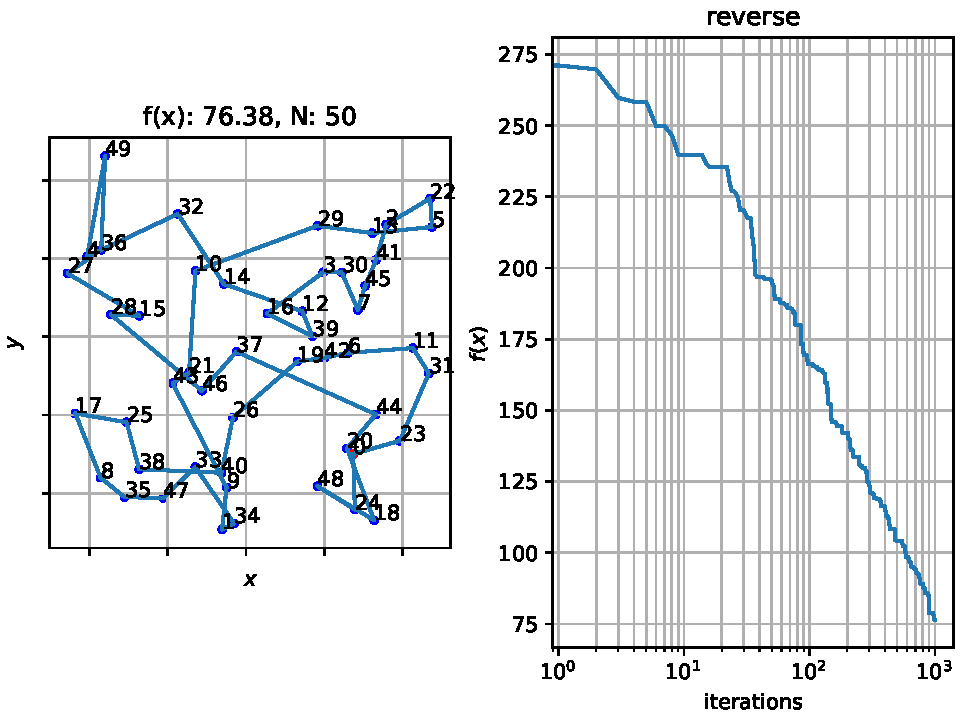
\includegraphics[width=0.49\textwidth]{rand-reverse}}
\caption{Local search algorithms performance on an instance of the problem}
\label{fig:res-local-search}
\end{figure}

\begin{figure}
\centering
\subfloat[\emph{Circular layout}]%
	{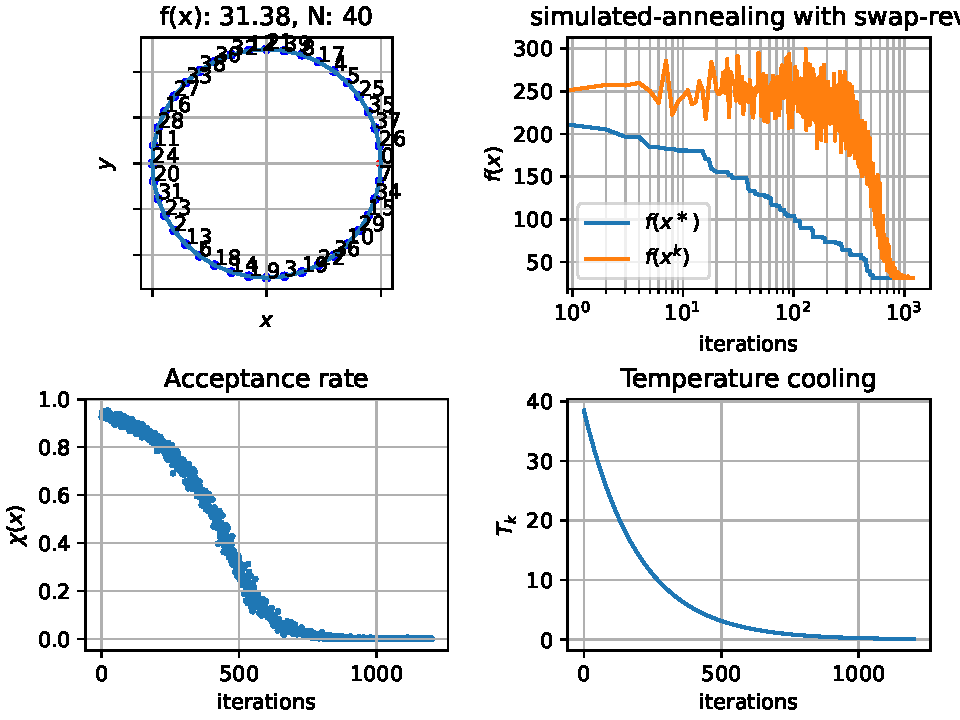
\includegraphics[width=0.49\textwidth]{circle-annealing-quad}} \,
\subfloat[\emph{Random layout}]%
	{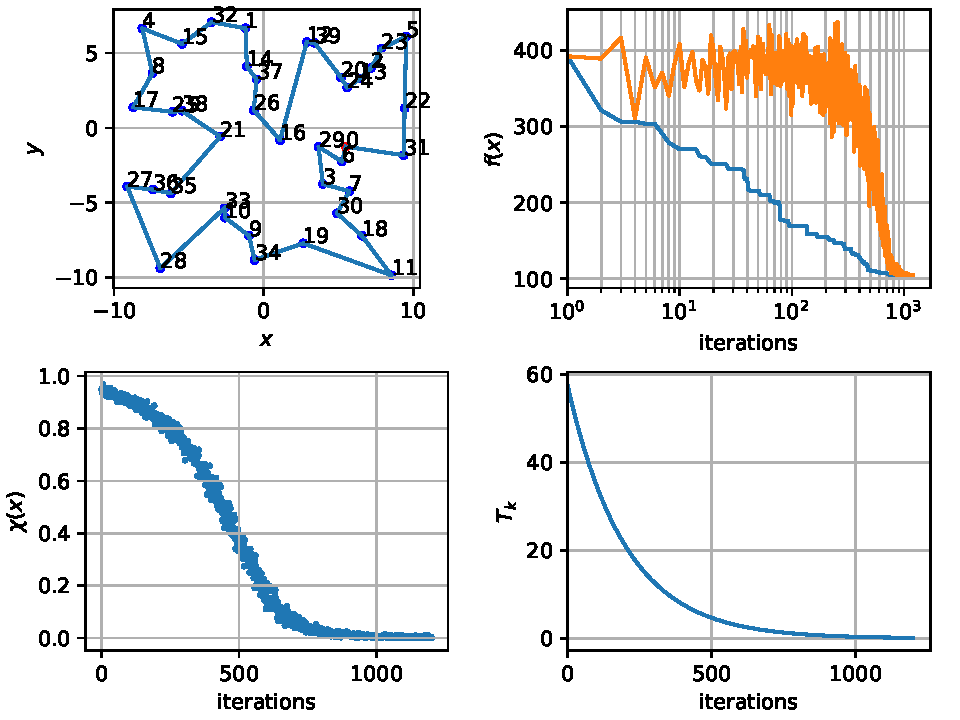
\includegraphics[width=0.49\textwidth]{rand-annealing-quad}}
\caption{Simulated annealing performance on a instance of the problem}
\label{fig:res-sim-annealing}
\end{figure}
